\documentclass{standalone}
\usepackage{tikz}
\usetikzlibrary{patterns, positioning}
\usepackage[sfdefault]{ClearSans} %% option 'sfdefault' activates Clear Sans as the default text font
\usepackage[T1]{fontenc}

\begin{document}
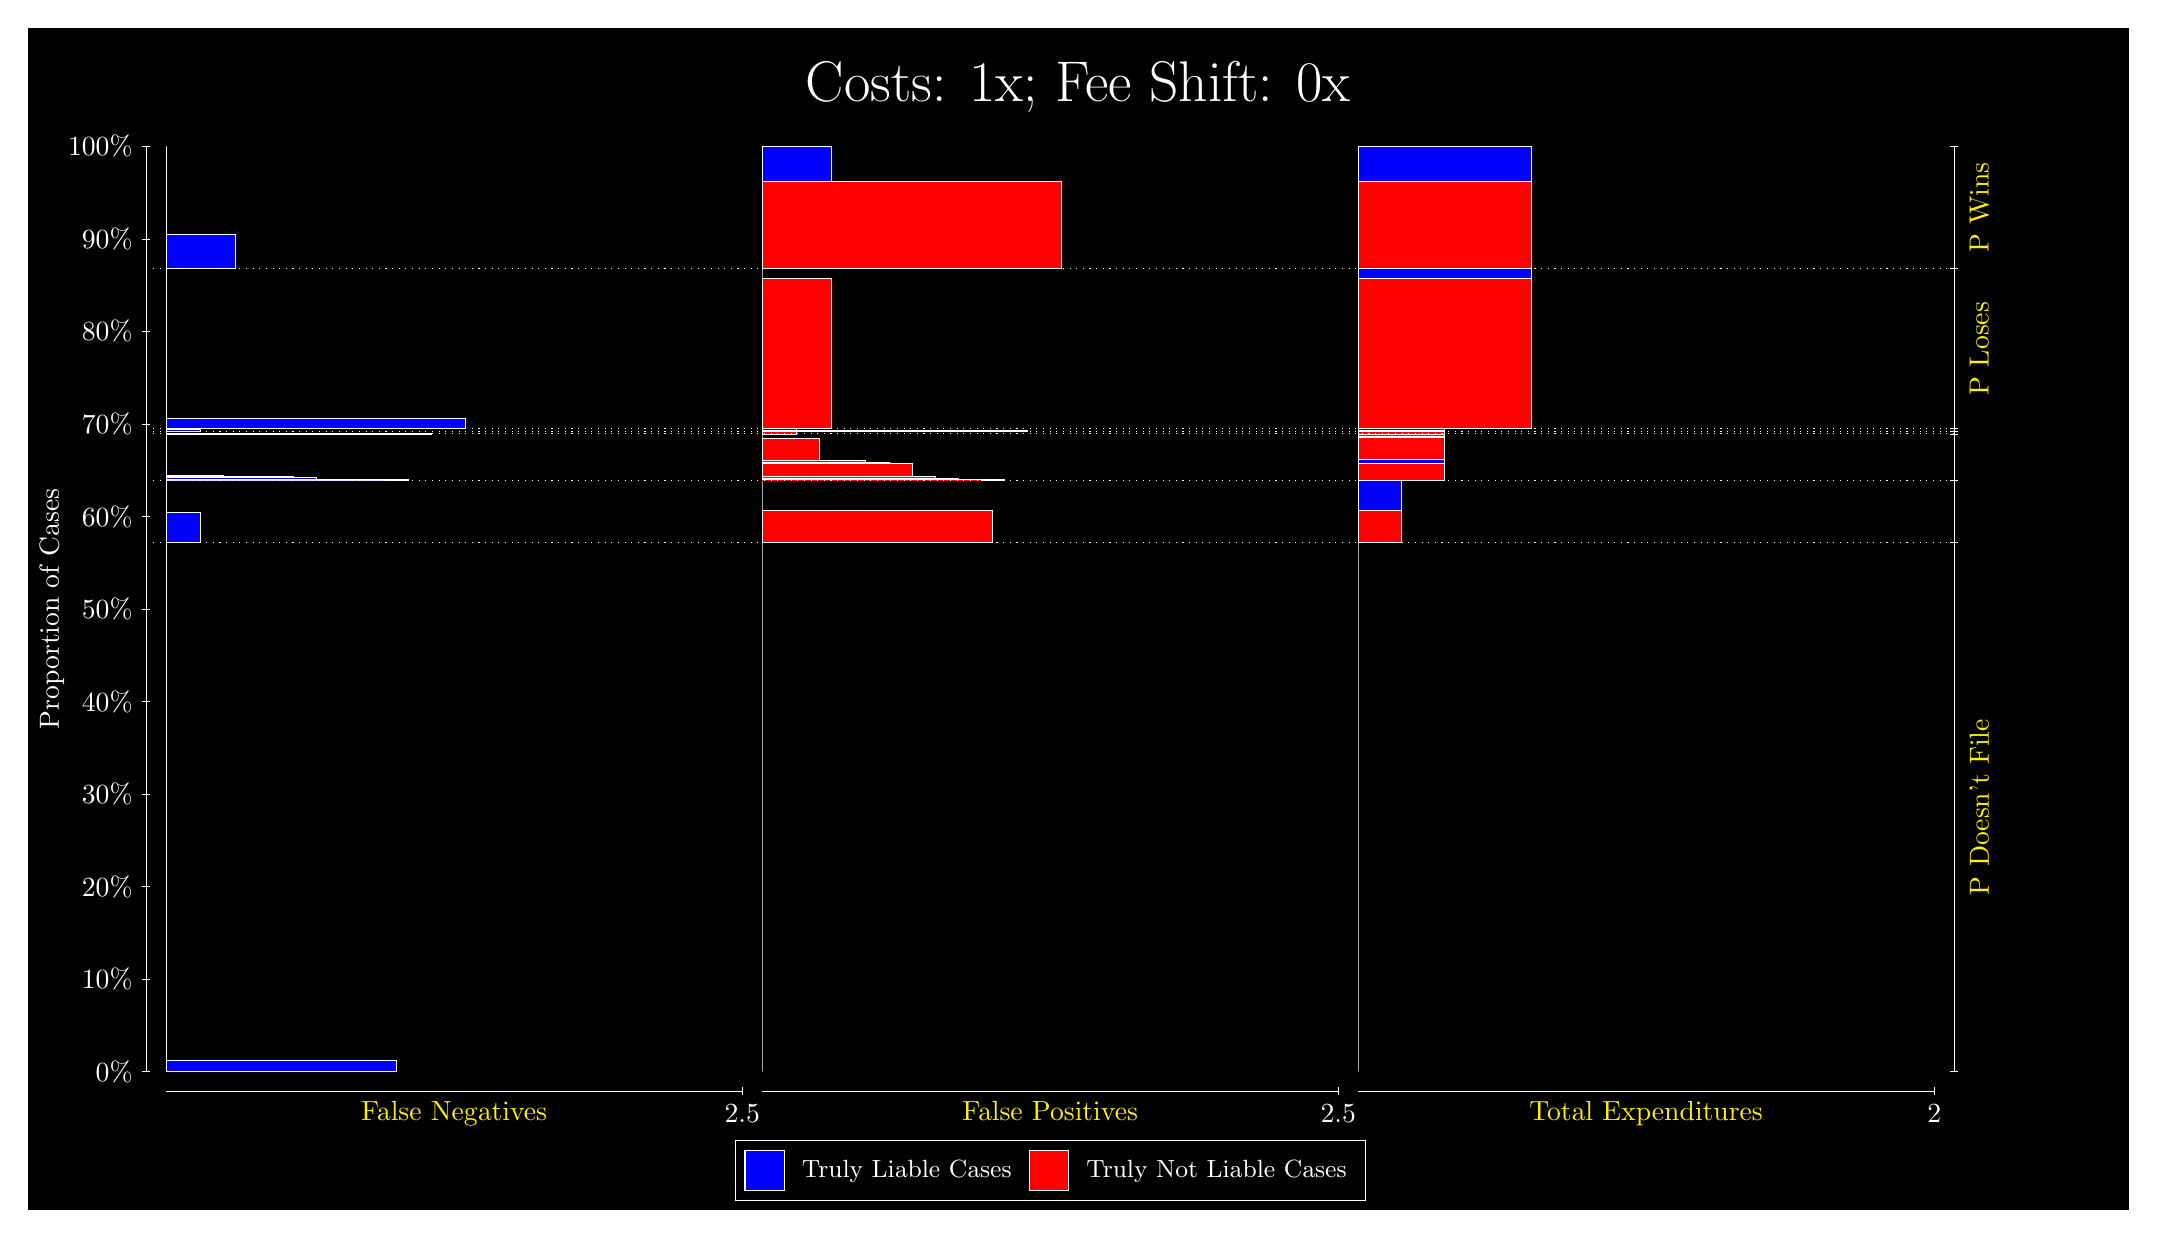
\begin{tikzpicture}
\draw[fill=black] (0,0) rectangle (26.667,15);
\draw[text=white] (0,13.5) rectangle (26.667,15) node[midway] {\huge Costs: 1x; Fee Shift: 0x};
\draw[white, very thin] (1.5,1.75) -- (1.5,13.5);
\node[rotate=90, text=white, anchor=center] at (0.3, 7.625) {Proportion of Cases};
\draw[white, very thin] (1.45,1.75) -- (1.55,1.75);
\node[text=white, anchor=east] at (1.45, 1.75) {0\%};
\draw[white, very thin] (1.45,2.925) -- (1.55,2.925);
\node[text=white, anchor=east] at (1.45, 2.925) {10\%};
\draw[white, very thin] (1.45,4.1) -- (1.55,4.1);
\node[text=white, anchor=east] at (1.45, 4.1) {20\%};
\draw[white, very thin] (1.45,5.275) -- (1.55,5.275);
\node[text=white, anchor=east] at (1.45, 5.275) {30\%};
\draw[white, very thin] (1.45,6.45) -- (1.55,6.45);
\node[text=white, anchor=east] at (1.45, 6.45) {40\%};
\draw[white, very thin] (1.45,7.625) -- (1.55,7.625);
\node[text=white, anchor=east] at (1.45, 7.625) {50\%};
\draw[white, very thin] (1.45,8.8) -- (1.55,8.8);
\node[text=white, anchor=east] at (1.45, 8.8) {60\%};
\draw[white, very thin] (1.45,9.975) -- (1.55,9.975);
\node[text=white, anchor=east] at (1.45, 9.975) {70\%};
\draw[white, very thin] (1.45,11.15) -- (1.55,11.15);
\node[text=white, anchor=east] at (1.45, 11.15) {80\%};
\draw[white, very thin] (1.45,12.325) -- (1.55,12.325);
\node[text=white, anchor=east] at (1.45, 12.325) {90\%};
\draw[white, very thin] (1.45,13.5) -- (1.55,13.5);
\node[text=white, anchor=east] at (1.45, 13.5) {100\%};

\draw[white, very thin] (24.457,1.75) -- (24.457,13.5);
\draw[white, very thin] (24.407,1.75) -- (24.507,1.75);
\node[anchor=west] at (24.407, 1.75) {};
\draw[white, very thin] (24.407,8.4661) -- (24.507,8.4661);
\node[anchor=west] at (24.407, 8.4661) {};
\draw[white, very thin] (24.407,9.2613) -- (24.507,9.2613);
\node[anchor=west] at (24.407, 9.2613) {};
\draw[white, very thin] (24.407,9.8488) -- (24.507,9.8488);
\node[anchor=west] at (24.407, 9.8488) {};
\draw[white, very thin] (24.407,9.8822) -- (24.507,9.8822);
\node[anchor=west] at (24.407, 9.8822) {};
\draw[white, very thin] (24.407,9.9196) -- (24.507,9.9196);
\node[anchor=west] at (24.407, 9.9196) {};
\draw[white, very thin] (24.407,11.946) -- (24.507,11.946);
\node[anchor=west] at (24.407, 11.946) {};
\draw[white, very thin] (24.407,13.5) -- (24.507,13.5);
\node[anchor=west] at (24.407, 13.5) {};

\draw[white, very thin, fill=blue] (1.75,1.75) rectangle (4.6775,1.8976);
\draw[white, very thin, fill=red] (1.75,1.8976) rectangle (1.75,8.4661);
\draw[white, very thin, fill=blue] (1.75,8.4661) rectangle (2.1891,8.8489);
\draw[white, very thin, fill=red] (1.75,8.8489) rectangle (1.75,9.2613);
\draw[white, very thin, fill=blue] (1.75,9.2613) rectangle (4.8239,9.2683);
\draw[white, very thin, fill=blue] (1.75,9.2683) rectangle (4.5312,9.2683);
\draw[white, very thin, fill=blue] (1.75,9.2683) rectangle (4.2384,9.2702);
\draw[white, very thin, fill=blue] (1.75,9.2702) rectangle (3.9457,9.2707);
\draw[white, very thin, fill=blue] (1.75,9.2707) rectangle (3.6529,9.2998);
\draw[white, very thin, fill=blue] (1.75,9.2998) rectangle (3.3602,9.3071);
\draw[white, very thin, fill=blue] (1.75,9.3071) rectangle (3.0674,9.3145);
\draw[white, very thin, fill=blue] (1.75,9.3145) rectangle (2.7746,9.3152);
\draw[white, very thin, fill=blue] (1.75,9.3152) rectangle (2.4819,9.3215);
\draw[white, very thin, fill=red] (1.75,9.3215) rectangle (1.75,9.8488);
\draw[white, very thin, fill=blue] (1.75,9.8488) rectangle (5.1167,9.8497);
\draw[white, very thin, fill=red] (1.75,9.8497) rectangle (1.75,9.8822);
\draw[white, very thin, fill=blue] (1.75,9.8822) rectangle (2.1891,9.9022);
\draw[white, very thin, fill=red] (1.75,9.9022) rectangle (1.75,9.9196);
\draw[white, very thin, fill=blue] (1.75,9.9196) rectangle (5.5558,10.042);
\draw[white, very thin, fill=red] (1.75,10.042) rectangle (1.75,11.946);
\draw[white, very thin, fill=blue] (1.75,11.946) rectangle (2.6283,12.387);
\draw[white, very thin, fill=red] (1.75,12.387) rectangle (1.75,13.5);
\draw[white, very thin, fill=red] (9.3189,1.75) rectangle (9.3189,8.3185);
\draw[white, very thin, fill=blue] (9.3189,8.3185) rectangle (9.3189,8.4661);
\draw[white, very thin, fill=red] (9.3189,8.4661) rectangle (12.246,8.8785);
\draw[white, very thin, fill=blue] (9.3189,8.8785) rectangle (9.3189,9.2613);
\draw[white, very thin, fill=red] (9.3189,9.2613) rectangle (12.393,9.2664);
\draw[white, very thin, fill=red] (9.3189,9.2664) rectangle (12.1,9.2673);
\draw[white, very thin, fill=red] (9.3189,9.2673) rectangle (11.807,9.2856);
\draw[white, very thin, fill=red] (9.3189,9.2856) rectangle (11.515,9.3133);
\draw[white, very thin, fill=red] (9.3189,9.3133) rectangle (11.222,9.4774);
\draw[white, very thin, fill=red] (9.3189,9.4774) rectangle (10.929,9.479);
\draw[white, very thin, fill=red] (9.3189,9.479) rectangle (10.929,9.4823);
\draw[white, very thin, fill=red] (9.3189,9.4823) rectangle (10.636,9.5079);
\draw[white, very thin, fill=red] (9.3189,9.5079) rectangle (10.344,9.508);
\draw[white, very thin, fill=red] (9.3189,9.508) rectangle (10.051,9.7886);
\draw[white, very thin, fill=blue] (9.3189,9.7886) rectangle (9.4652,9.795);
\draw[white, very thin, fill=blue] (9.3189,9.795) rectangle (9.3189,9.8488);
\draw[white, very thin, fill=red] (9.3189,9.8488) rectangle (9.758,9.8813);
\draw[white, very thin, fill=blue] (9.3189,9.8813) rectangle (9.3189,9.8822);
\draw[white, very thin, fill=red] (9.3189,9.8822) rectangle (12.686,9.8996);
\draw[white, very thin, fill=blue] (9.3189,9.8996) rectangle (9.758,9.9196);
\draw[white, very thin, fill=red] (9.3189,9.9196) rectangle (10.197,11.823);
\draw[white, very thin, fill=blue] (9.3189,11.823) rectangle (9.3189,11.946);
\draw[white, very thin, fill=red] (9.3189,11.946) rectangle (13.125,13.059);
\draw[white, very thin, fill=blue] (9.3189,13.059) rectangle (10.197,13.5);
\draw[white, very thin, fill=red] (16.888,1.75) rectangle (16.888,8.3185);
\draw[white, very thin, fill=blue] (16.888,8.3185) rectangle (16.888,8.4661);
\draw[white, very thin, fill=red] (16.888,8.4661) rectangle (17.437,8.8785);
\draw[white, very thin, fill=blue] (16.888,8.8785) rectangle (17.437,9.2613);
\draw[white, very thin, fill=red] (16.888,9.2613) rectangle (17.986,9.479);
\draw[white, very thin, fill=blue] (16.888,9.479) rectangle (17.986,9.53);
\draw[white, very thin, fill=red] (16.888,9.53) rectangle (17.986,9.8106);
\draw[white, very thin, fill=blue] (16.888,9.8106) rectangle (17.986,9.8175);
\draw[white, very thin, fill=red] (16.888,9.8175) rectangle (17.986,9.8465);
\draw[white, very thin, fill=blue] (16.888,9.8465) rectangle (17.986,9.8488);
\draw[white, very thin, fill=red] (16.888,9.8488) rectangle (17.986,9.8813);
\draw[white, very thin, fill=blue] (16.888,9.8813) rectangle (17.986,9.8822);
\draw[white, very thin, fill=red] (16.888,9.8822) rectangle (17.986,9.8996);
\draw[white, very thin, fill=blue] (16.888,9.8996) rectangle (17.986,9.9196);
\draw[white, very thin, fill=red] (16.888,9.9196) rectangle (19.083,11.823);
\draw[white, very thin, fill=blue] (16.888,11.823) rectangle (19.083,11.946);
\draw[white, very thin, fill=red] (16.888,11.946) rectangle (19.083,13.059);
\draw[white, very thin, fill=blue] (16.888,13.059) rectangle (19.083,13.5);
\draw[white, dotted] (1.5,8.4661) -- (24.457,8.4661);
\draw[white, dotted] (1.5,9.2613) -- (24.457,9.2613);
\draw[white, dotted] (1.5,9.8488) -- (24.457,9.8488);
\draw[white, dotted] (1.5,9.8822) -- (24.457,9.8822);
\draw[white, dotted] (1.5,9.9196) -- (24.457,9.9196);
\draw[white, dotted] (1.5,11.946) -- (24.457,11.946);
\draw[white, very thin] (1.75,1.5) -- (9.0689,1.5);
\node[text=yellow, anchor=north] at (5.4094, 1.5) {False Negatives};
\draw[white, very thin] (9.0689,1.45) -- (9.0689,1.55);
\node[text=white, anchor=north] at (9.0689, 1.45) {2.5};

\draw[white, very thin] (9.3189,1.5) -- (16.638,1.5);
\node[text=yellow, anchor=north] at (12.978, 1.5) {False Positives};
\draw[white, very thin] (16.638,1.45) -- (16.638,1.55);
\node[text=white, anchor=north] at (16.638, 1.45) {2.5};

\draw[white, very thin] (16.888,1.5) -- (24.207,1.5);
\node[text=yellow, anchor=north] at (20.547, 1.5) {Total Expenditures};
\draw[white, very thin] (24.207,1.45) -- (24.207,1.55);
\node[text=white, anchor=north] at (24.207, 1.45) {2};

\node[text=yellow, centered, rotate=90] at (24.777, 5.108) {P Doesn't File};




\node[text=yellow, centered, rotate=90] at (24.777, 10.933) {P Loses};
\node[text=yellow, centered, rotate=90] at (24.777, 12.723) {P Wins};

\draw (12.978300999999998,1.5) node[draw=none] (baseCoordinate) {};
\begin{scope}[align=center]
        \matrix[scale=0.5, draw=white, below=0.5cm of baseCoordinate, nodes={draw}, column sep=0.1cm]{
            \node[rectangle, draw, minimum width=0.5cm, minimum height=0.5cm, fill=blue] {}; &
            \node[draw=none, font=\small, text=white] (B) {Truly Liable Cases}; &
            \node[rectangle, draw, minimum width=0.5cm, minimum height=0.5cm, fill=red] {}; &
            \node[draw=none, font=\small, text=white] (B) {Truly Not Liable Cases}; \\
            };
\end{scope}

\end{tikzpicture}
\end{document}